\section{Metadata Analysis and Findings}
\label{sec:metadata}

We start our analysis by exploring the key metadata attributes associated with the publications. Specifically, we focus on metadata associated with publications authors and their respective institutes, before inspecting the structural elements of the articles (e.g., presence of equations). In this section we focus on comparing these observations across the all venues under study. 

\subsection{Research Productivity of Authors and Countries}

\vspace{2mm}
\subsubsection{Author Based Productivity Analysis}

First, we investigate the most important authors of the our dataset. \ignacio{May be use a quantile to define top} There are many parameters to analyze the significance of a researcher's published work. 


\begin{figure}[H]
	\begin{center}
		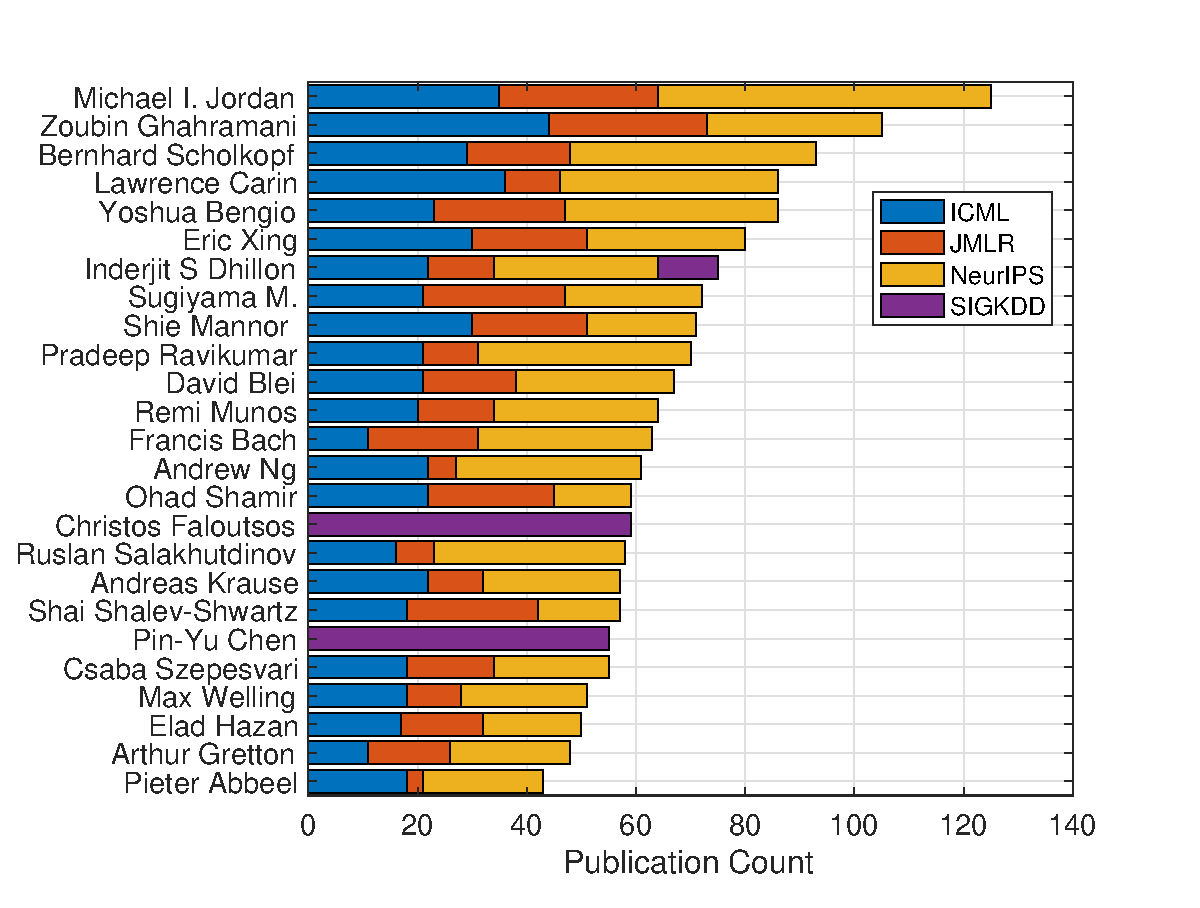
\includegraphics[width=0.45\textwidth]{figure/Total_pub_auth.eps}
	\end{center}
	\caption{Authors with the highest publication count during 2004--2019. \textit{Most of the authors are performing equally well in ICML, JMLR, and NeurIPS but have not published a single paper in SIGKDD.}}
% 	\ignacio{change legend to SIGKDD}}}
	\label{fig:author_total}
\end{figure}

A simple measure would be publication count,  as listed in Figure \ref{fig:author_total}. Most of the authors are performing equally well in ICML, JMLR, and NeurIPS but have not published a single paper in SIGKDD. Only two of the top author have focally published in SIGKDD. Inderjit S. Dhillon is the only author who have performed equally well across all of the understudy venues. Figure \ref{fig:authors_top} also shows the top authors individually in all of the four venues.
% \gareth{Could we add another fig next to Fig 2? This would be a 4xCDFs showing the distribution of papers-per-author across the entire dataset. This would provide context for this top 25 list (i.e. I'm guessing most authors only have 1 paper)}

\begin{figure*}[!htpb]
	\begin{center}
			\subfloat[]{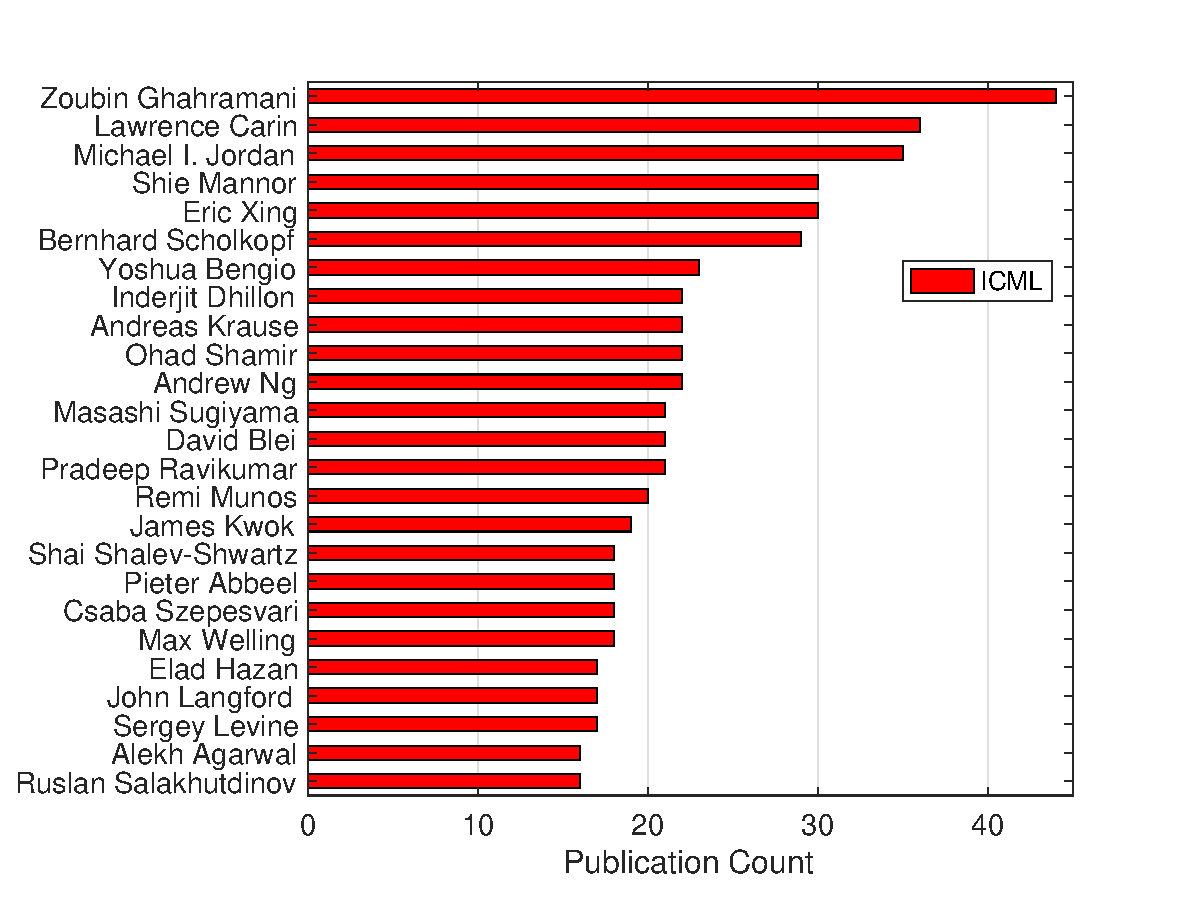
\includegraphics[width=0.45\textwidth]{figure/Freq_ICML.eps}}
	\subfloat[]{\includegraphics[width=0.45\textwidth]{figure/authors_freq_JMLR.eps}}\\
		\subfloat[]{\includegraphics[width=0.45\textwidth]{figure/author_freq_NIPS.eps}}
	\subfloat[]{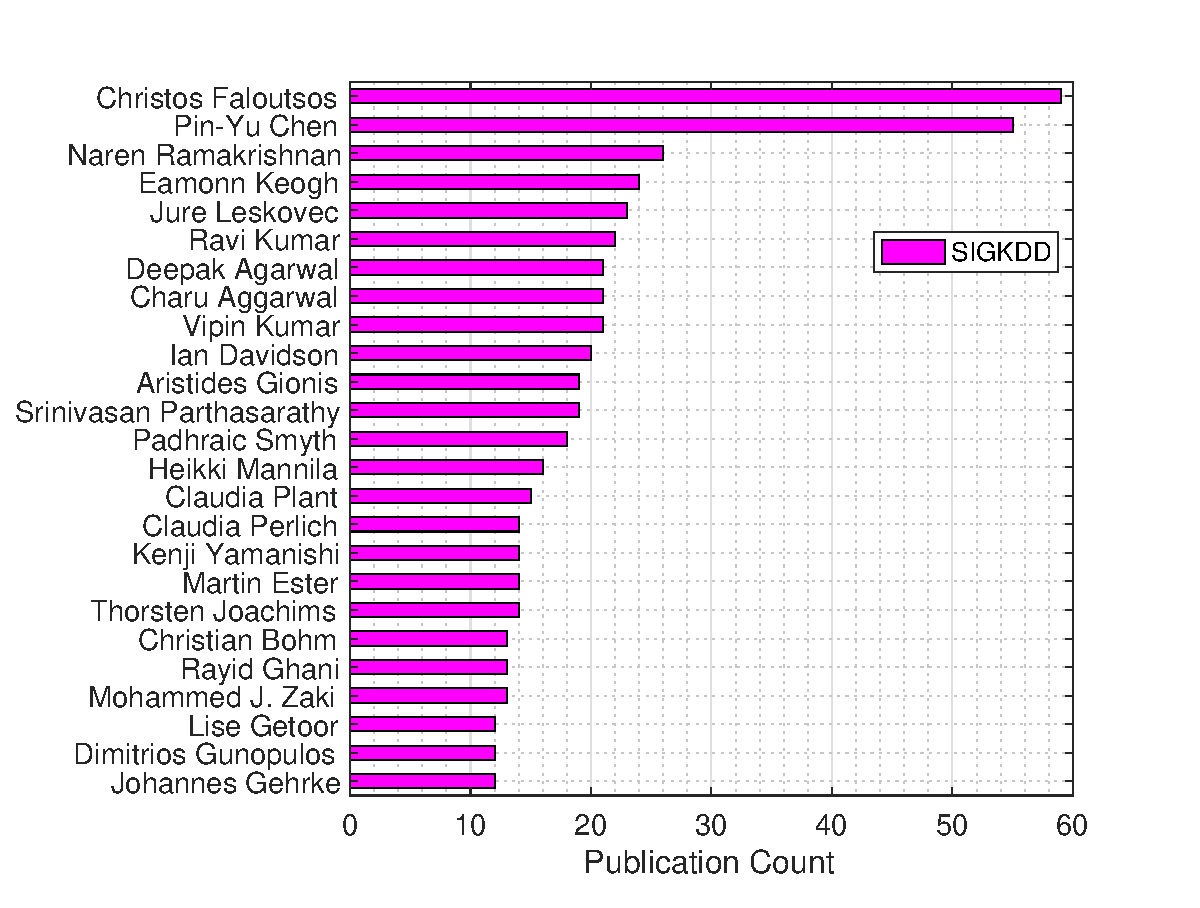
\includegraphics[width=0.45\textwidth]{figure/Author_freq_SIGKDD.eps}}
	\end{center}
	\caption{Most-published authors during 2004--2019, according to article count. \textit{Interestingly, there are major overlap in theoretical study based articles, supporting a ``Renaissance Man'' hypothesis implying that there are many authors who are equally extremely prolific across the theoretical studies based venues.}}
	\label{fig:authors_top}
\end{figure*}

\begin{figure*}[!htbp]
	\begin{center}
		\subfloat[]{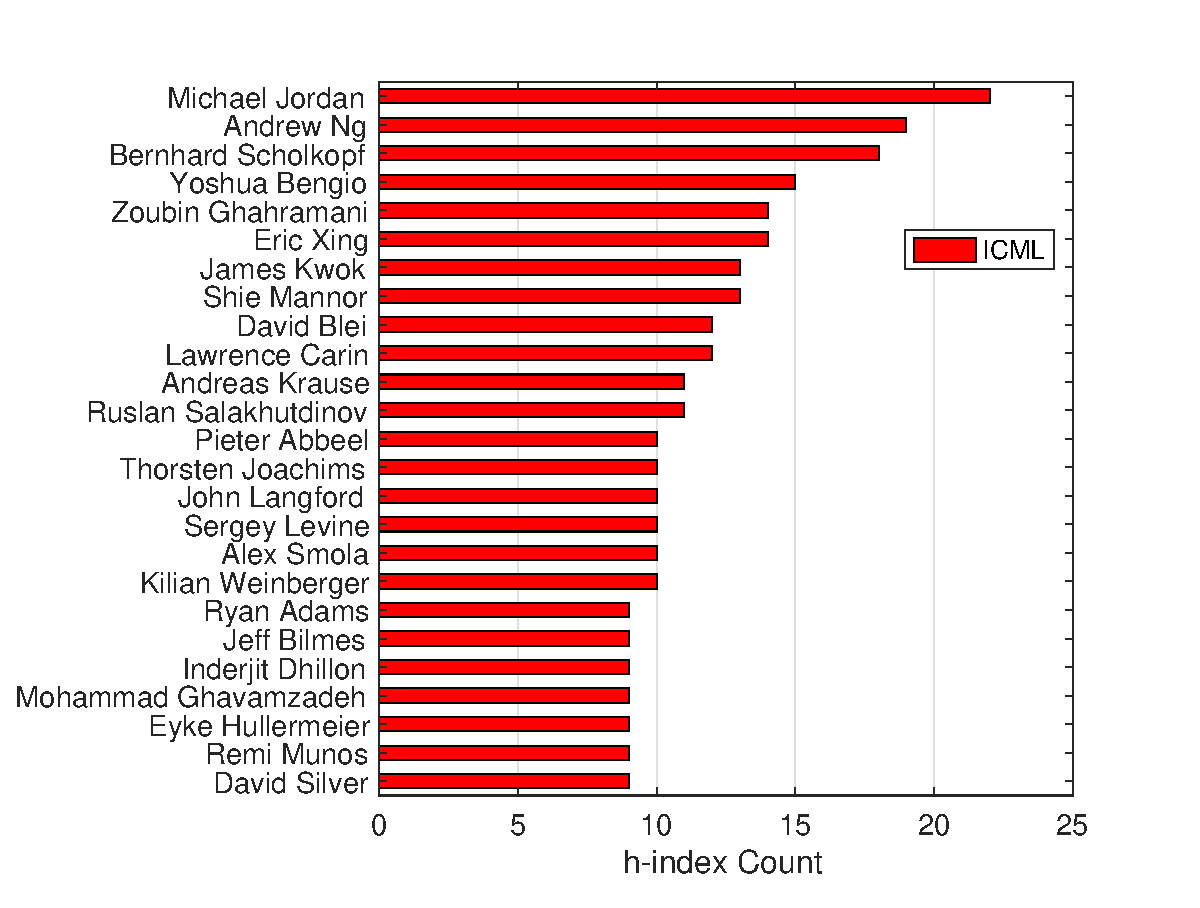
\includegraphics[width=0.45\textwidth]{figure/h-index_ICML.eps}}
	\subfloat[]{\includegraphics[width=0.45\textwidth]{figure/authors_freq_hindex_JMLR.eps}}\\
		\subfloat[]{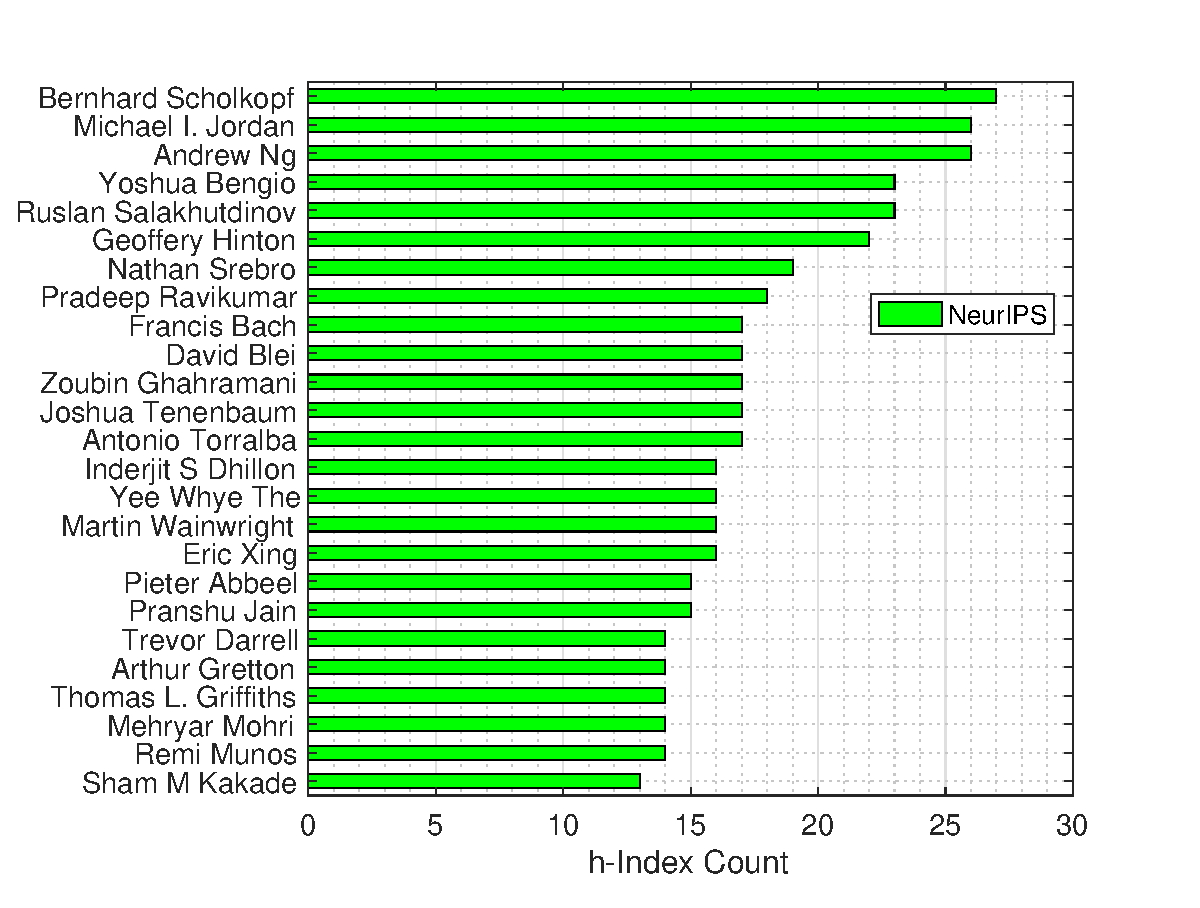
\includegraphics[width=0.45\textwidth]{figure/auth_h-index_NIPS.eps}}
	\subfloat[]{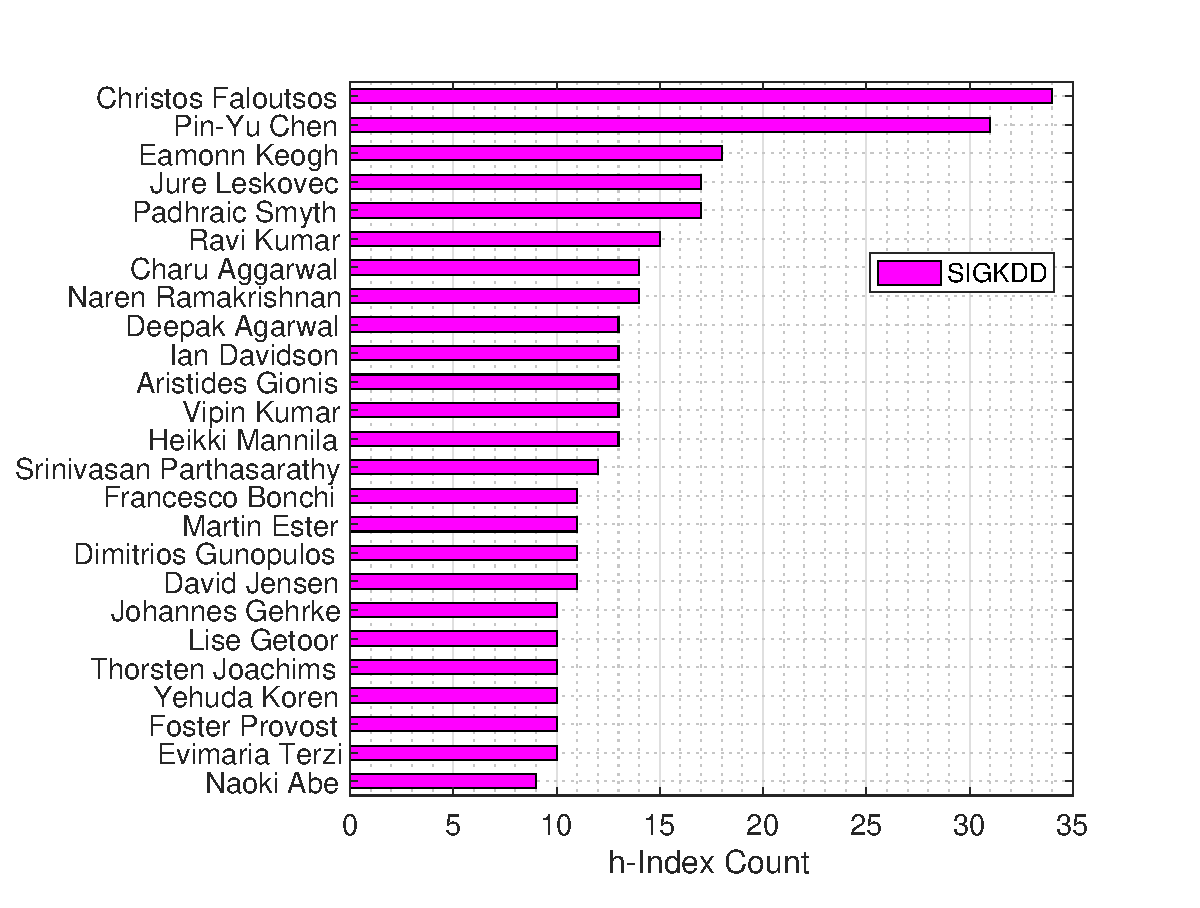
\includegraphics[width=0.45\textwidth]{figure/Author_hindex_SIGKDD.eps}}
	\end{center}
	\caption{Authors with the highest h-index during 2004--2019. \textit{The most-published list and authors with the highest h-index are almost identical in both machine learning and neural networks based studies (i.e. ICML, JMLR, and NeurIPS) indicating a strong relationship between numbers of articles published and h-index. Similar trend is also observed in SIGKDD as well.}}
	\label{fig:cited_top_hindex}
\end{figure*}


The h-index is also another widely used metric where \textit{h} tells us that \textit{h} articles of a researcher have \textit{h} citations \citep{hirsch2005index}. Using the h-index of only ICML, JMLR, NeurIPS, and SIGKDD, we can observe which authors are publishing highly cited research in these venues. 
Figure \ref{fig:cited_top_hindex} shows the authors in our dataset with the highest h-index, and how the top highest publication counts are from the authors with the highest h-index across all discussed genre of articles. The data confirms that the top authors (measured by publication count) are the ones who have significant research contributions in terms of publication count as well as citation count.



\subsubsection{Country Based Productivity Analysis}

In a research domain, some countries play a pivotal role in driving the ongoing advancements in that field. Figure \ref{fig:country_top} shows the rank of different countries based on published articles in all of the four datasets using a global heat map. 


Data shows that the United States and United Kingdom are in the first two highest position in all four venues in terms of publication count. Other top countries include Canada, China, France, and the Germany in all of the four venues. This trend shows that only a handful of countries are contributing disproportionately in development of machine learning research. There is an absence of scholarship from Africa in all of these venues where as Afro-ethnic researcher are contributing quality research with affiliation of other countries in all of the four venues. Similarly, NeurIPS is not geographically diverse as other countries.


The differences in a country's publications in the various venues can partly be attributed to different publication cultures arising from different incentives for faculty promotion/assessment. Some countries in North America and parts of Europe (e.g., USA and UK) give more weight to top-tier conferences (like ICML, NeurIPS etc.) in their assessment criteria while many others in parts of Asia and southern Europe (e.g., India, Malaysia, France, Spain, Italy) emphasize journal publications. In many cases, extended versions of conference papers in the machine learning domain are published in journals such as JMLR.

\begin{figure*}[!htbp]
	\centering
	\subfloat[]{\includegraphics[width=0.45\textwidth]{figure/ICML_full_final.png}}
	\subfloat[]{\includegraphics[width=0.45\textwidth]{figure/JMLR_Full_final.png}}\\
		\subfloat[]{\includegraphics[width=0.45\textwidth]{figure/NeuIPS_Full_final.png}}
	\subfloat[]{\includegraphics[width=0.45\textwidth]{figure/SIGKDD_full_final.png}}
	\caption{Rank of different countries based on publication count in all of four venues. \textit{Although most countries have similar productivity in these venues, there are notable exceptions where the publication trends are quite dissimilar.}}
	\label{fig:country_top}
\end{figure*}

From the above analysis, it is evident that all of the four venues attract attention from significant researchers in the field. Hence, we posit that it may be difficult for new emerging scholars to publish in such venues. 
Indeed, anecdotally, this is often claimed.
To identify emerging authors, we extract all papers with: $(i)$ authors who have never published in the venue before; and $(ii)$ authors who do not have any co-authors who have already published in the venue. 
Figure \ref{fig:country_emer} shows the distribution of emerging authors in all venues conferences during 2004--2019.


\begin{figure*}[!htbp]
	\centering
	\subfloat[]{\includegraphics[width=0.45\textwidth]{figure/ICML_emer_final.png}}
	\subfloat[]{\includegraphics[width=0.45\textwidth]{figure/JMLR_emer_final.png}}\\
		\subfloat[]{\includegraphics[width=0.45\textwidth]{figure/NeurIPS_emer_final.png}}
	\subfloat[]{\includegraphics[width=0.45\textwidth]{figure/SIGKDD_emer_final.png}}
	\caption{Rank of different countries based on publication count from first-time contributor in all of four venues. \textit{ Those include $(i)$ authors who have never published in the venue before; and $(ii)$ authors who do not have any co-authors who have already published in the venue.}}
	\label{fig:country_emer}
\end{figure*}

\begin{figure*}[!htbp]
	\centering
	\subfloat[]{\includegraphics[width=0.45\textwidth]{figure/COUNTRY_GRAPH_ICML_u.png}}
	\subfloat[]{\includegraphics[width=0.45\textwidth]{figure/country_al.png}}\\
		\subfloat[]{\includegraphics[width=0.45\textwidth]{figure/countries_NIPS.png}}
	\subfloat[]{\includegraphics[width=0.45\textwidth]{figure/Country_SIGKDD.png}}
	\caption{Co-authorship network among top countries in (a) ICML; (b) JMLR; (c) NeurIPS; and (d) SIGKDD. Node size indicates the number of links with other nodes in the co-authorship network and the node color represents cluster membership.}
	\label{fig:country_top_gephi}
\end{figure*}


We next inspect the collaborations that took place between these countries. Figure \ref{fig:country_top_gephi} shows the co-authorship network of top countries in all four venues. 

In ICML, JMLR, and NeurIPS, the top five countries have significant co-authorship activities among themselves, thus they are clustered in a single group. In SIGKDD, top publishing are clustered in two clusters. With the advancement of information and communication technologies, researchers from various countries now have new ways to work with each other. Top countries enjoy the share of publication from their authors, and in addition a contribution from authors from collaborating countries. 




\subsubsection{Institutional and Author Based Collaborations}
This subsection presents the varying trends of collaborations among the institutes and authors in ICML, JMLR, NeurIPS, and SIGKDD over the period from 2004 to 2019. We will address several important questions relating to the collaboration patterns of institutes and countries; the most influential institutes and authors in all of the four venues; and whether influential institutes and authors tend to work as collaborators. To observe collaborative relations among the top researchers in all of four venues, we generate undirected graphs of co-authors and identify clusters using modularity class partitioning. We used undirected graphs to remove duplicate links among publishing entities. 

Figure \ref{fig:authors_top_gephi} presents the clusters present in the network. We find 187 different clusters of authors in ICML, 31 clusters in JMLR, 145 clusters in NeurIPS, and 83 clusters in SIGKDD. To improve the visualization, we only include authors who have more than five articles in ICML, JMLR, NeurIPS, and SIGKDD. 


\begin{figure*}[!htbp]
	\centering
	\subfloat[]{\includegraphics[width=0.45\textwidth]{figure/authors_graph_ICML_u.png}}
	\subfloat[]{\includegraphics[width=0.45\textwidth]{figure/authors_graph_JMLR_u.png}}\\
		\subfloat[]{\includegraphics[width=0.45\textwidth]{figure/auth_AL_NIPS_u.png}}
	\subfloat[]{\includegraphics[width=0.45\textwidth]{figure/authors_al_SIGKDD.png}}
	\caption{Co-authorship network among top authors in the field of machine learning (a) ICML; (b) JMLR; (c) NeurIPS; and (d) SIGKDD. Only those who have authored at least 5 articles are kept in clusters.}
	\label{fig:authors_top_gephi}
\end{figure*}


Published research is a crucial factor in determining the quality of education and research at any institute. Figure \ref{fig:inst_top} shows a similar result for the top institutes. We performed a clustering analysis using modularity class algorithm over ICML, JMLR, NeurIPS, and SIGKDD articles. 

Figure \ref{fig:inst_top_gephi} shows a similar result for all of the four venues datasets. In all venues, the top publishing institutes are clustered into three groups according to their publishing behavior. In all of the four venues, CMU, UC Berkeley, Stanford University, and MIT, both in the United States, showed a significant co-authorship pattern. 



\begin{figure*}[!htbp]
	\begin{center}
		\subfloat[]{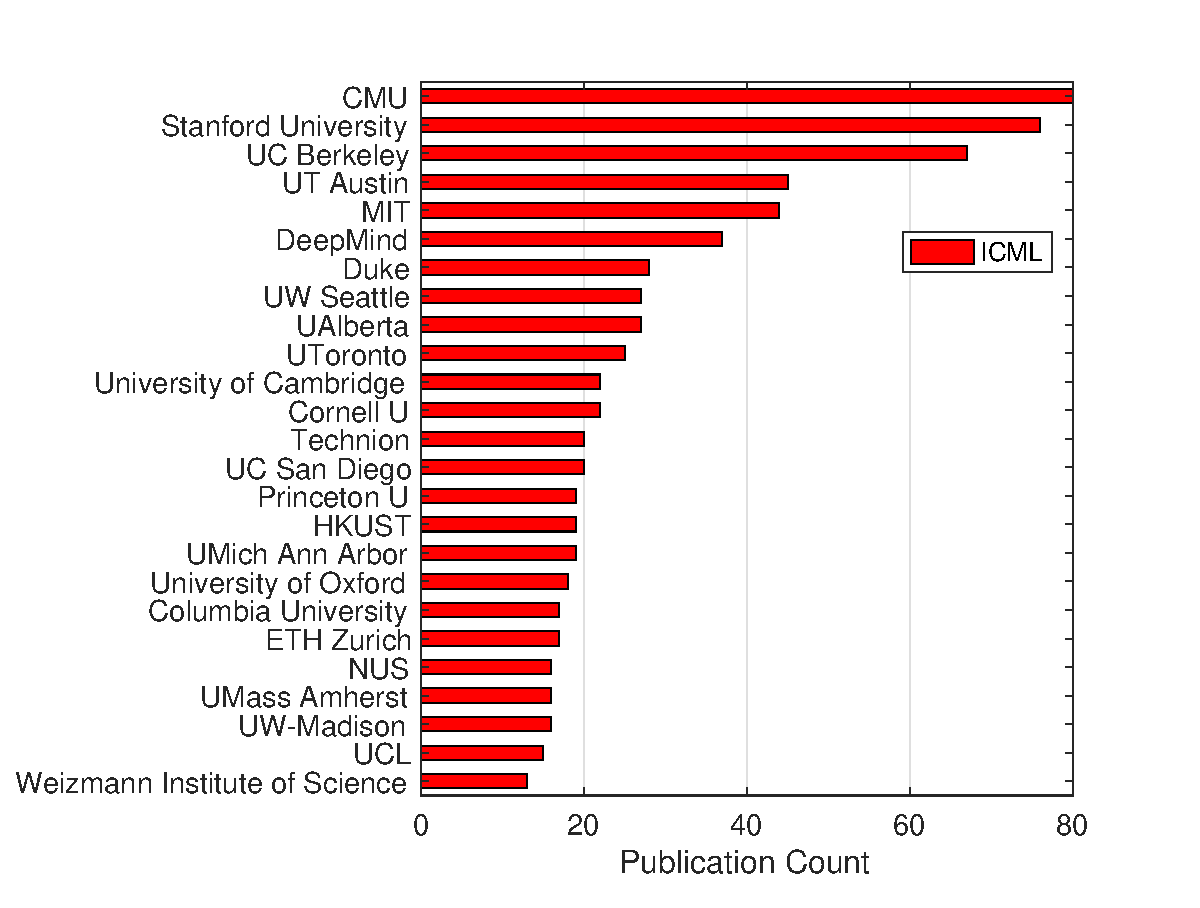
\includegraphics[width=0.45\textwidth]{figure/Insti_Freq_ICML.eps}}
	\subfloat[]{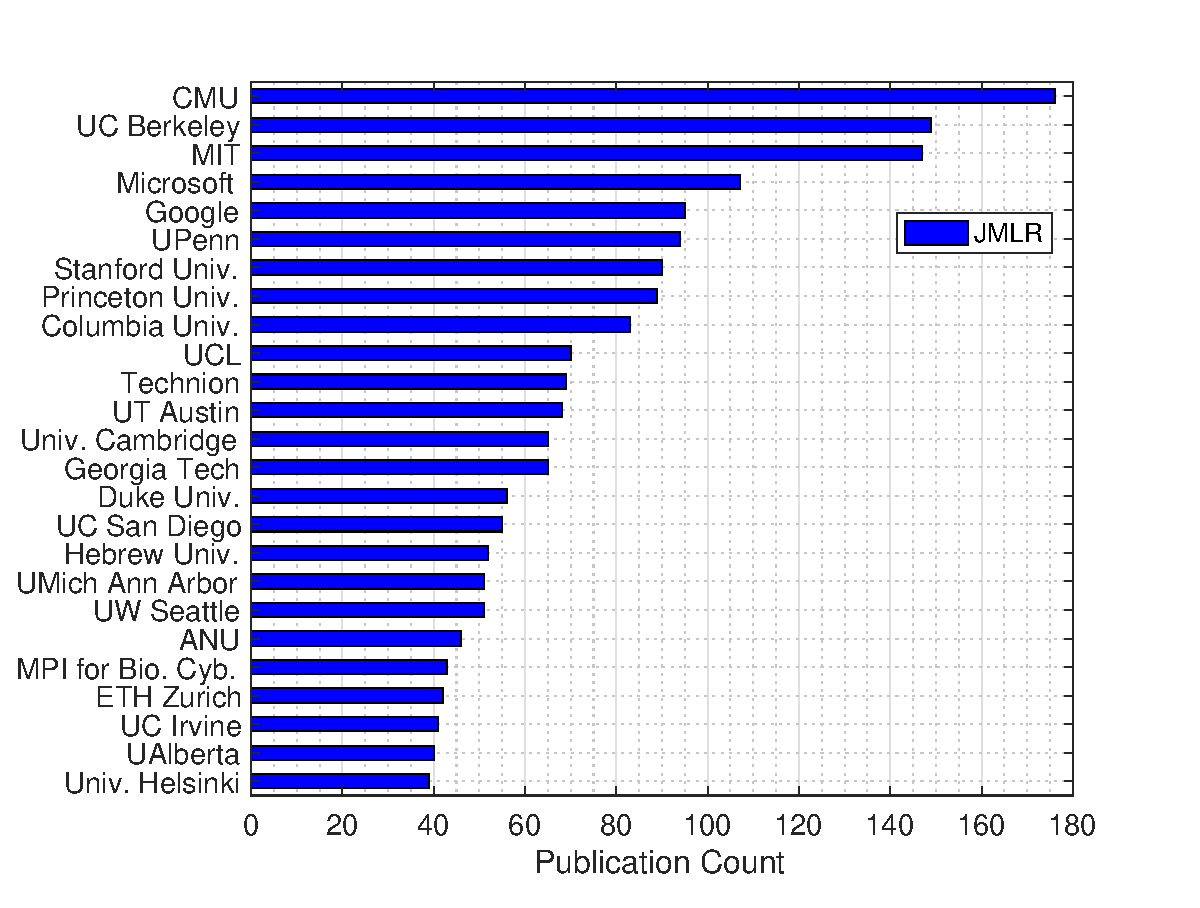
\includegraphics[width=0.45\textwidth]{figure/institutes_freq_JMLR.eps}}\\
		\subfloat[]{\includegraphics[width=0.45\textwidth]{figure/institutes_NIPS.eps}}
	\subfloat[]{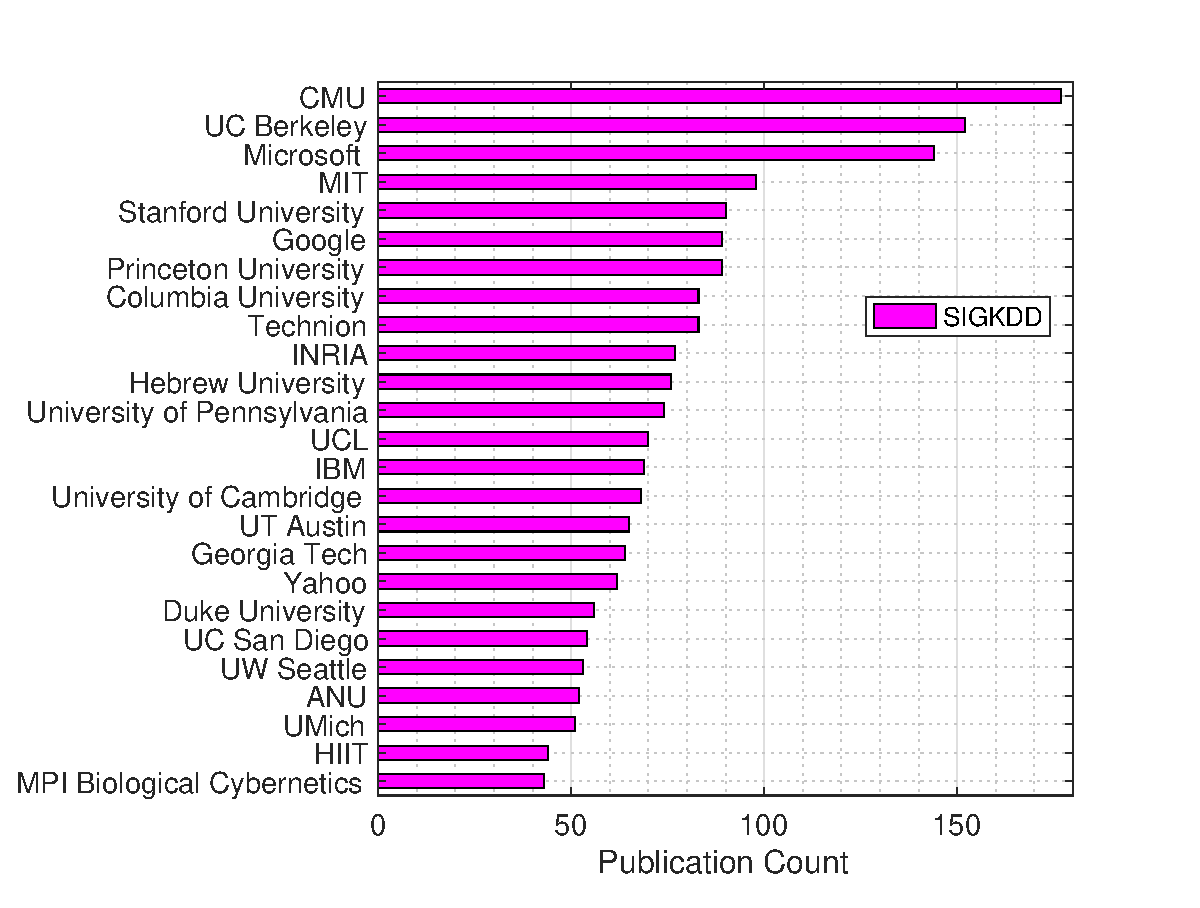
\includegraphics[width=0.45\textwidth]{figure/Institutes_freq_SIGKDD.eps}}
	\end{center}
	\caption{Most-published institutes during 2004--2019, according to their article count. \textit{In all of the four venues, academic institutes are publishing more significant contributors as compared industrial contributors. CMU tops all four venues followed by Stanford in two venues and by UC Berkeley in the other two venues.}}
	\label{fig:inst_top}
\end{figure*}


\begin{figure*}[!htbp]
	\centering
	\subfloat[]{\includegraphics[width=0.45\textwidth]{figure/insti_graph_ICML.png}}
	\subfloat[]{\includegraphics[width=0.45\textwidth]{figure/institute_al_JMLR_u_al.png}}\\
		\subfloat[]{\includegraphics[width=0.45\textwidth]{figure/institutes_NIPS_u_al.png}}
	\subfloat[]{\includegraphics[width=0.45\textwidth]{figure/Institutes_SIGKDD_u_al.png}}
	\caption{Co-authorship network among top institutes in (a) ICML; (b) JMLR; (c) NeurIPS; and (d) SIGKDD (with 10 minimum published articles). \textit{Distinct patterns can be observed in all four venues: academic institutes are prominent in all across the dataset.}}
	\label{fig:inst_top_gephi}
\end{figure*}

To remove the weak links, in all venues we set the degree threshold to 10. We found 21 different clusters of institutes in ICML, 84 clusters in JMLR, 42 clusters in NeurIPS, and 29 clusters in SIGKDD. To improve the visualization, we only include institutes who have more than 10 articles in all four venues. Social network analysis has shown us the hidden relations between the top authors of ICML, JMLR, NeurIPS, and SIGKDD, and we conclude that most of the top authors (measured by their publication count in all four venues) are clustered together because either they have strong collaboration behavior with each other or common co-author in-between.

\subsection{Referencing Patterns}
First, we extract the references from all papers and create a citation graph, as we are curious to understand how all ICML, JMLR, NeurIPS, and SIGKDD cite each other.
Figure \ref{fig:top_flow_venues_c} is a Sankey diagram, showing the fraction of papers that reference papers from all of the four venues (left), as well as the other papers that in turn cite the papers in our dataset (right). 

Note that this covers all of the four venues. 
Interesting patterns emerge from this analysis. 
Most noteworthy is the bias for citing papers from the same venue. For example, 26\% of references in ICML papers are for other papers previously published in ICML. Similar trend are observed for other venues as well. 


In contrast, a far more diverse body of publication outlets list papers from our dataset in their references. This is particularly for other conferences (57\% of the papers in our dataset which cite our selected venues are actually conferences, rather than journals). 
Major citers of our dataset papers include Neurocomputing, ICLR, CVPR, and IEEE Access.
This trend is perhaps intuitive as all of the four venues are considered among the most prestigious outlets, and therefore it is unsurprising that a wide diversity of venues cite such papers. 
All that said, it is clear that a number of other publication venues feature heavily in the bibliographies of our dataset's papers, and these are dominated by conferences rather than journals.


\begin{figure}[H]
	\centering
	\includegraphics[width=0.45\textwidth]{figure/sanky_all.png}
	\caption{The distribution of references and citations in ICML, JMLR, NeurIPS, and SIGKDD. The left input shows the conferences that are referenced by all of the four venue papers; the right output shows which papers cite papers from our dataset. \emph{Major source of references and citations in our dataset are from conferences.} }
	\label{fig:top_flow_venues_c}
\end{figure}




\section{Content Based Analysis and Findings}
\label{sec:content}

This section keyword-based analysis, based on index keywords; We address questions such as, what topics are discussed by top authors in all of the four venues?

\subsection{Keyword-based analysis of articles} 



Investigating the popular topics is considered to be one of the best ways of studying the paradigm shifts in any research field. 
\begin{figure*}[!htbp]
	\begin{center}
		\subfloat[]{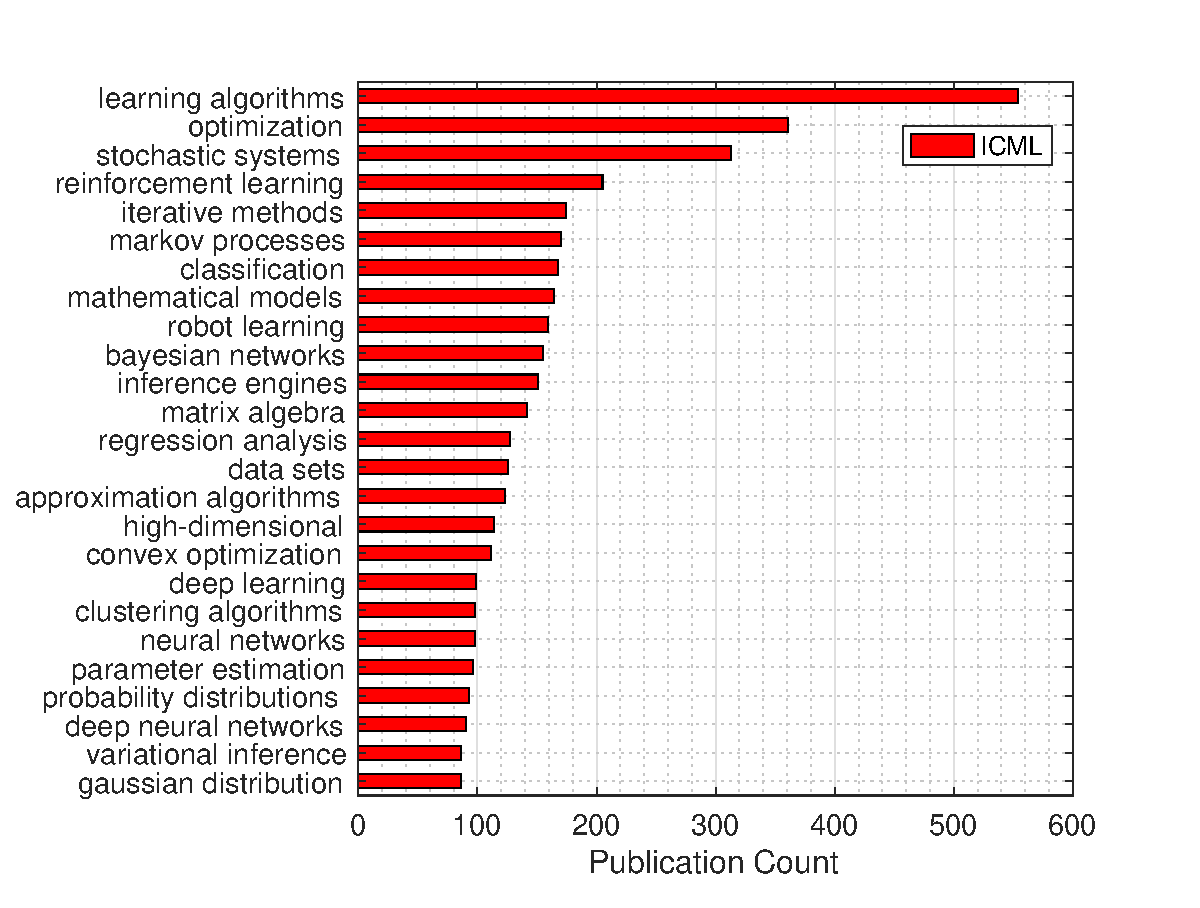
\includegraphics[width=0.45\textwidth]{figure/ICML_Keyword_Freq.eps}}
	\subfloat[]{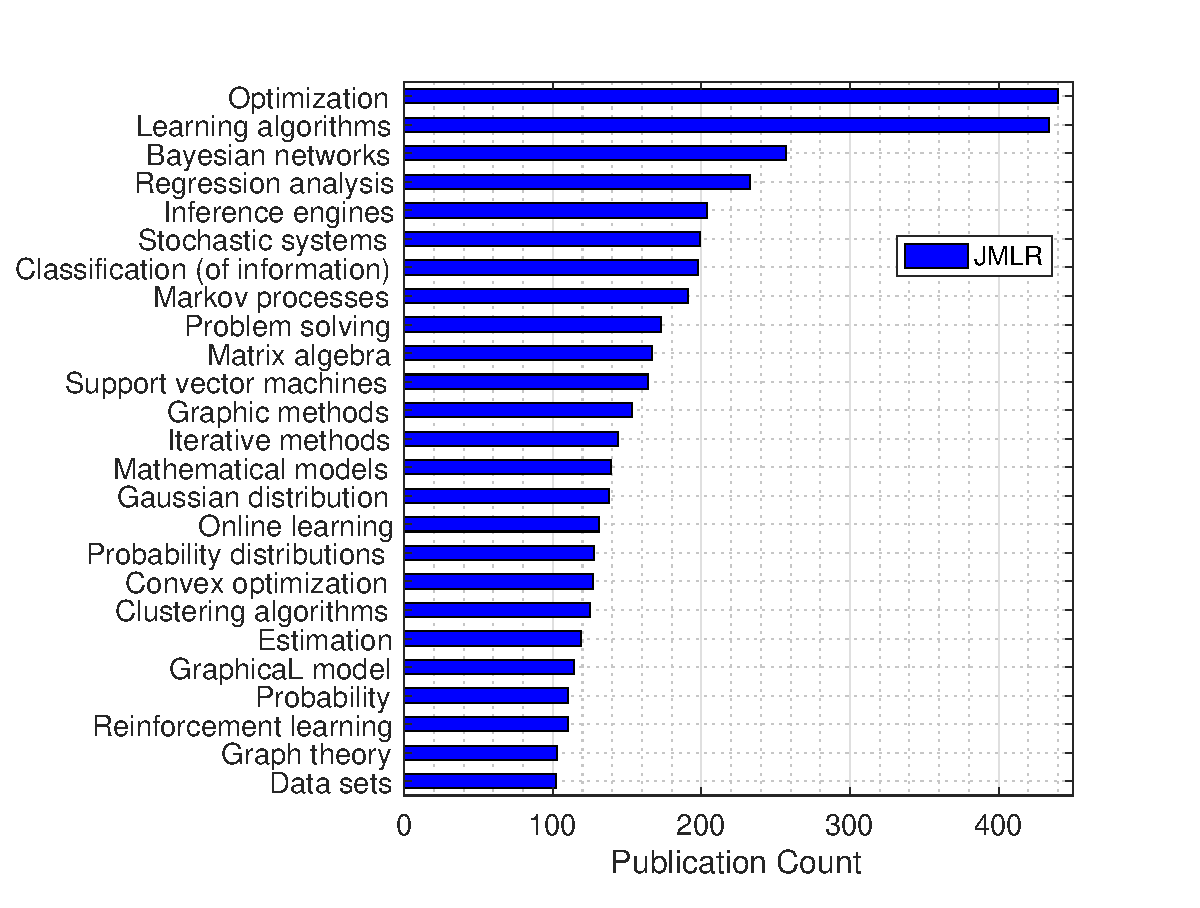
\includegraphics[width=0.45\textwidth]{figure/keywords_freq_JMLR.eps}}\\
		\subfloat[]{\includegraphics[width=0.45\textwidth]{figure/keyword_freq_NIPS.eps}}
	\subfloat[]{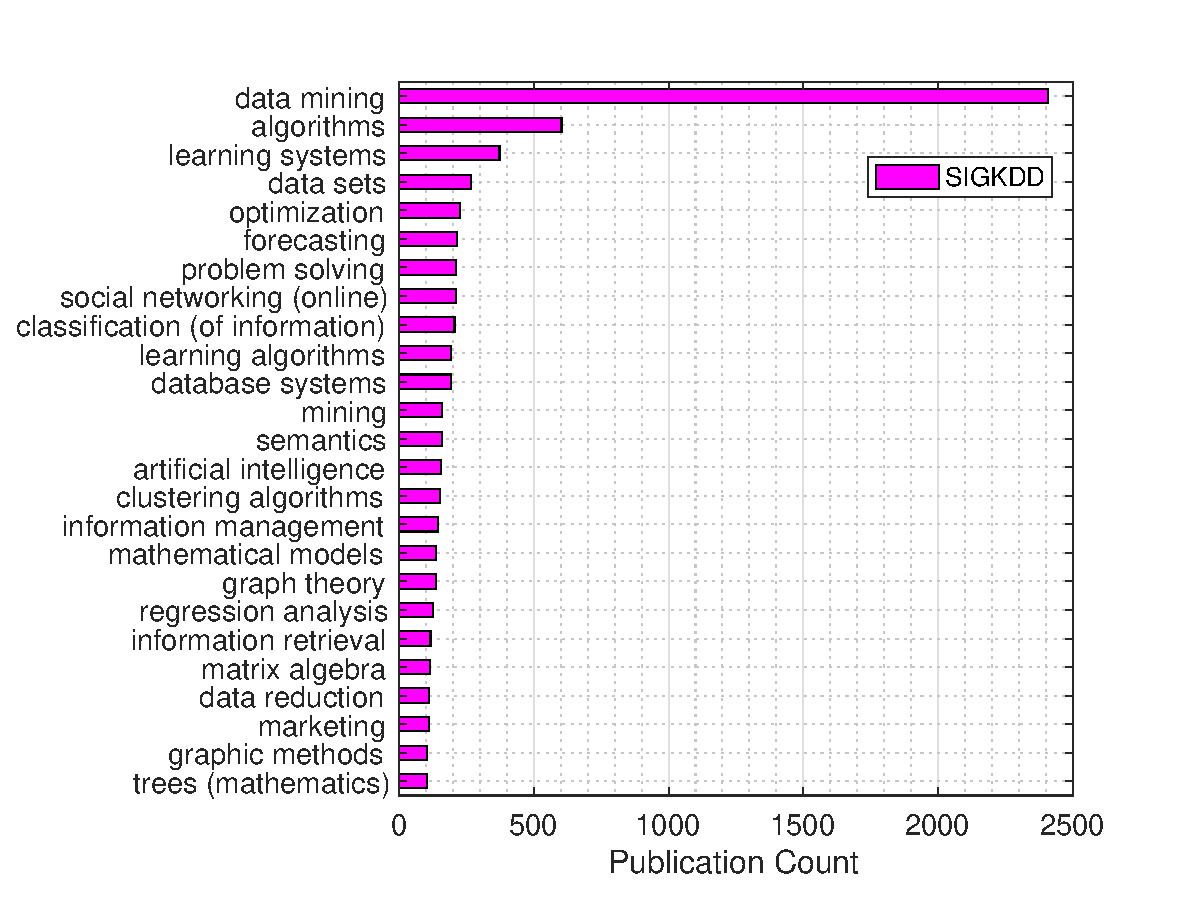
\includegraphics[width=0.45\textwidth]{figure/Keyword_freq_SIGKDD.eps}}
	\end{center}
	\caption{Most popular topics in ICML, JMLR, NeurIPS, and SIGKDD and their article count during 2004--2019, in terms of article count (cf. Figure \ref{fig:cited_top_keywords}, in which keywords of the most-cited articles are listed.)}
	\label{fig:keywords_top}
\end{figure*}

It is helpful in describing the research trends of a field. In this sub-section, we use ICML, JMLR, NeurIPS, and SIGKDD data to analyze the popular topics in the field of machine learning. We have described the top popular topics discussed in these articles in machine learning. This approach provides a holistic overview of research trends in machine learning since it covers both theoretical and application based articles.

Figure \ref{fig:keywords_top} represents the most popular topics in machine learning, according to the our dataset. ``Learning Systems'', ``Learning Algorithms'', ``Optimization'', and ``Data mining''. 


\subsection{Keyword co-occurrence analysis}
Keyword co-occurrence analysis helps researchers to find a publication venue's most common topics. 
\begin{figure*}[!htbp]
	\centering
	\subfloat[]{\includegraphics[width=0.45\textwidth]{figure/keyword_wo_large_ICML_u.png}}
	\subfloat[]{\includegraphics[width=0.45\textwidth]{figure/keyword_al_JMLR_u.png}}\\
		\subfloat[]{\includegraphics[width=0.45\textwidth]{figure/keyword_al_NIPS_u.png}}
	\subfloat[]{\includegraphics[width=0.45\textwidth]{figure/keyword_al_SIGKDD_u.png}}
	\caption{Keyword co-occurrence network in which the node size indicates the number of links with other nodes and node color represents cluster membership. \textit{It can be noted that keywords, discussed in our dataset, are typically biased towards algorithms and optimization (solutions and techniques)}.}
	\label{fig:keyword_top_gephi}
\end{figure*}

These analyses also help researchers to find topics and domains that are strongly related to each other. Figure \ref{fig:keyword_top_gephi} is the term co-occurrence map for ICML, JMLR, NeurIPS, and SIGKDD.

There is major overlap in the keywords used in the top-cited articles in all of the four venues. Keywords, discussed in our dataset, are typically biased towards algorithms and optimization (solutions and techniques).

Terms in a larger font size have a higher co-occurrence than other keywords in the graphs. In our dataset, frequently co-occurring terms are "Learning algorithms", "Optimization", "data mining", and "stochastic systems". Top keywords (measured on publication count) in our dataset are clustered in the same groups and have stronger links with each other than with unpopular keywords. This trend shows that in all of the four venues, there are only some top keywords (measured on publication count) which are discussed in most of the articles.



\section{Citation Based Analysis and Findings}
\label{sec:citation}

Citations are used to investigate the contributions of an author, organization, country or publication venue. Citation analysis is an effective tool to rank the productivity of various research bodies. In this section, we address some important bibliometric questions using citation data from ICML, JMLR, NeurIPS, and SIGKDD articles, such as who are the most-cited authors in all of the four venues; whether they have the same h-index as the most-published authors; whether increasing the number of authors affects the number of citations of an article; the most-cited keywords in all of the four venues.


\subsection{Citation Based Analysis of Different Research Entities}
In machine learning, some authors play more significant roles in advancements of the field than others. It is worth observing the impact and usability of their research. 
\begin{figure*}[!htbp]
	\begin{center}
	\subfloat[]{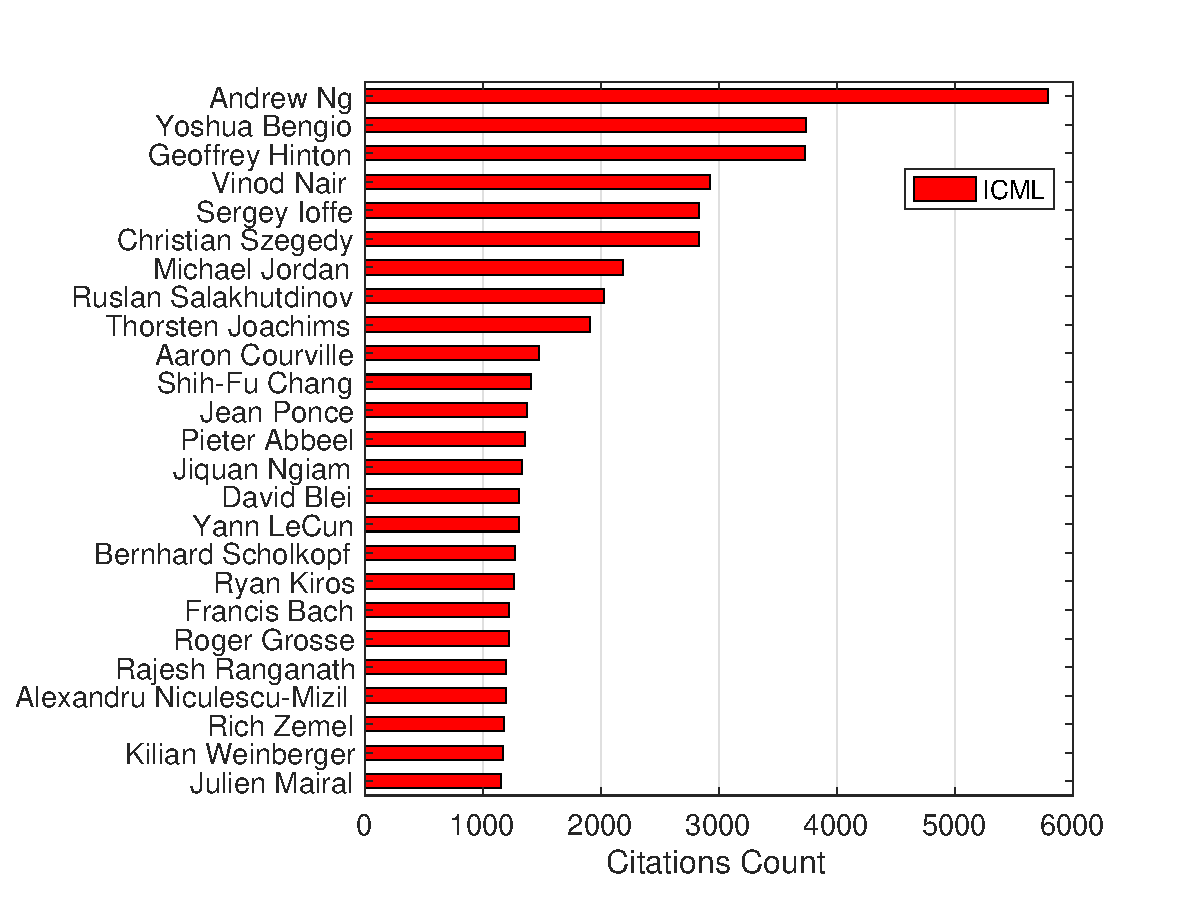
\includegraphics[width=0.45\textwidth]{figure/cite_ICML.eps}}
	\subfloat[]{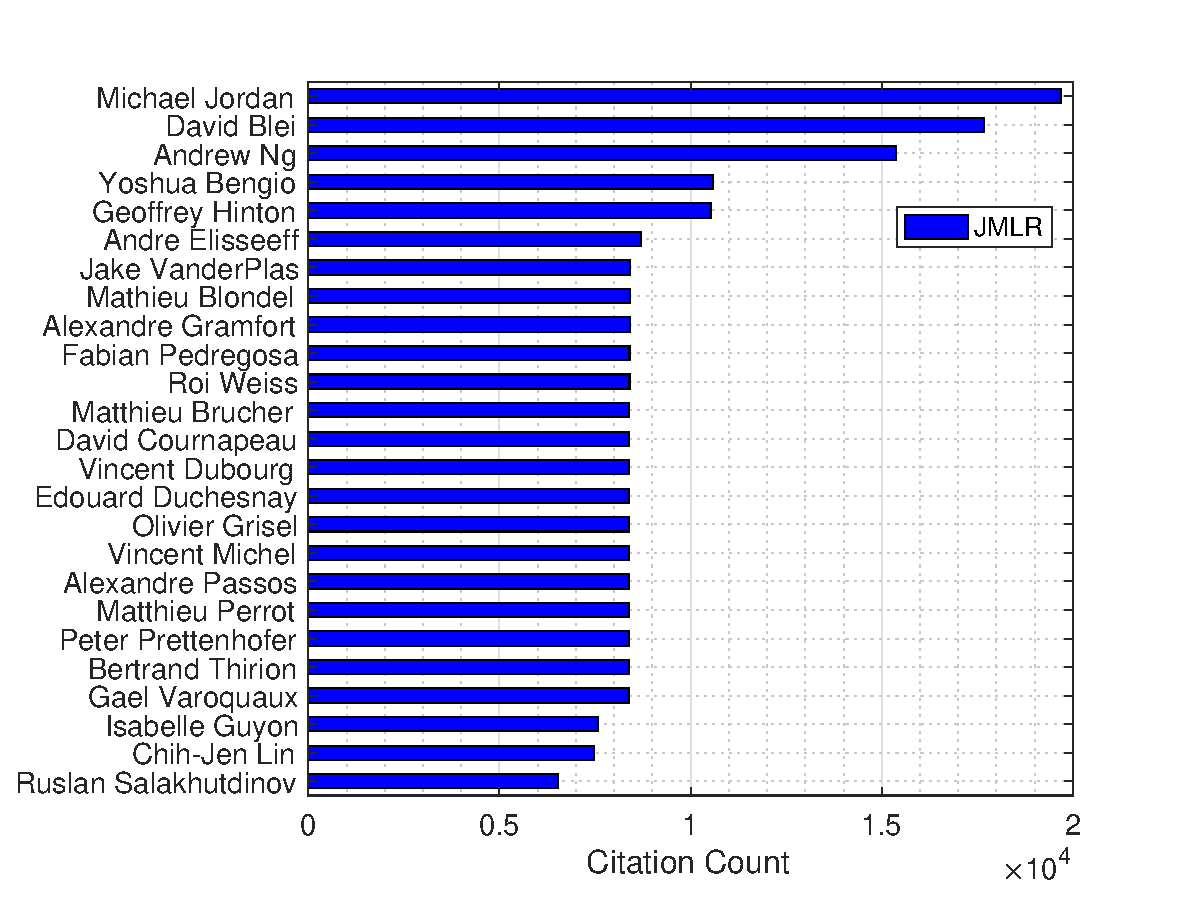
\includegraphics[width=0.45\textwidth]{figure/authors_freq_cite_JMLR.eps}}\\
		\subfloat[]{\includegraphics[width=0.45\textwidth]{figure/authors_cite_NIPS.eps}}
	\subfloat[]{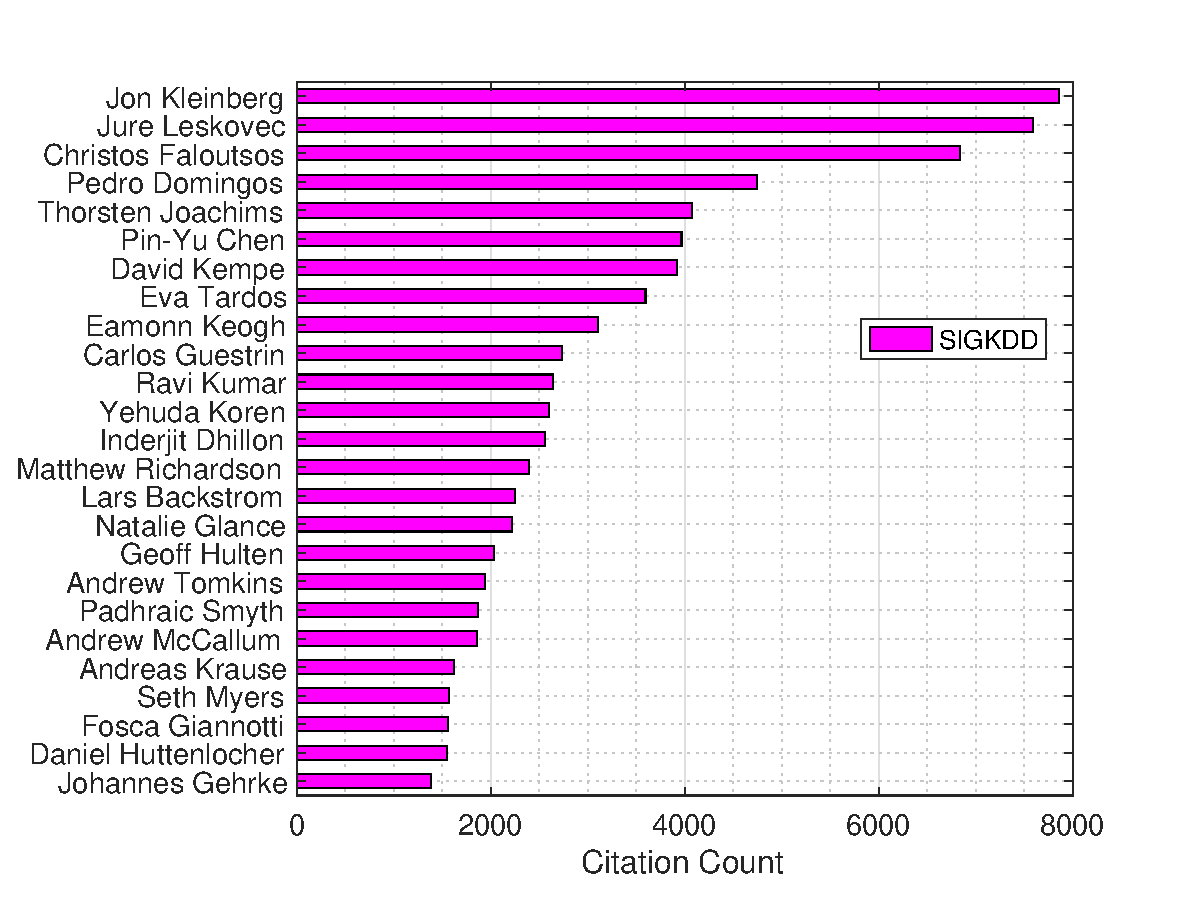
\includegraphics[width=0.45\textwidth]{figure/Author_cite_SIGKDD.eps}}
	\end{center}
	\caption{Most-cited authors. \textit{We see that the most-cited NeurIPS articles tend to have more citations as compared to other three venues.}}
	\label{fig:cited_top}
\end{figure*}


Figure \ref{fig:cited_top} shows the most-cited authors in all four venues from 2004 to 2019. From Figure \ref{fig:cited_top} and Figure \ref{fig:authors_top}, it can be observed that the top most-published authors and the top most-cited authors in all four venues are significantly different. 

Citations do not entirely represent the significance of the research undertaken by a researcher. There are many parameters to analyze its significance, but the h-index is the most widely used, and it is a better measure of an author's significance in a field than a simple citation count. 

Figure \ref{fig:cited_top_hindex} shows the authors in ICML, JMLR, NeurIPS, and SIGKDD with the highest h-index, and how the top highest publication counts are from the top authors with the highest h-index in all four venues. The data confirms that the top authors (measured by publication count) are the ones who have significant research contributions in terms of publication count as well as citation count.

Figure \ref{fig:cited_top_keywords} shows the most cited keywords in our dataset. We can observe that most cited keywords in all of the four venues are significantly different from most published ones.

\begin{figure*}[!htbp]
	\begin{center}
		\subfloat[]{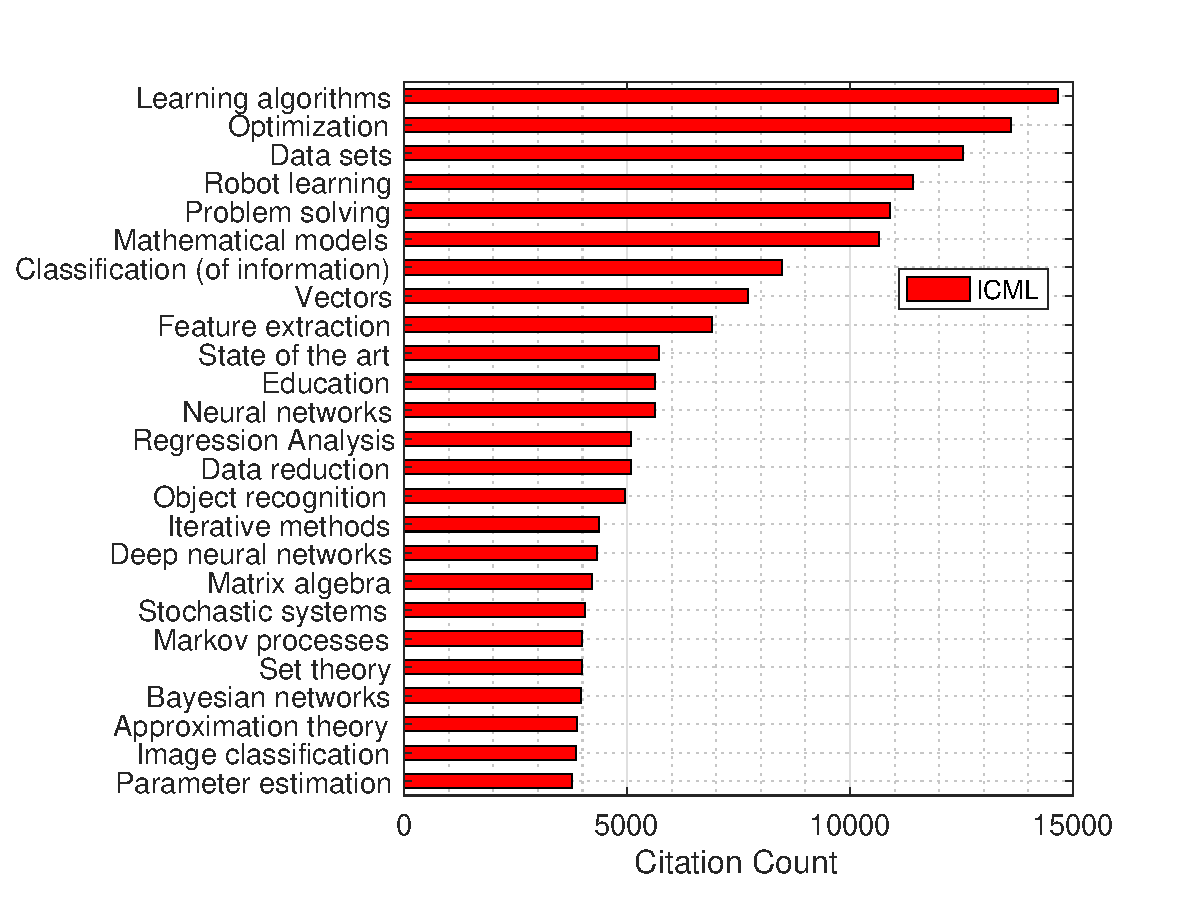
\includegraphics[width=0.45\textwidth]{figure/ICML_keyword_cite.eps}}
	\subfloat[]{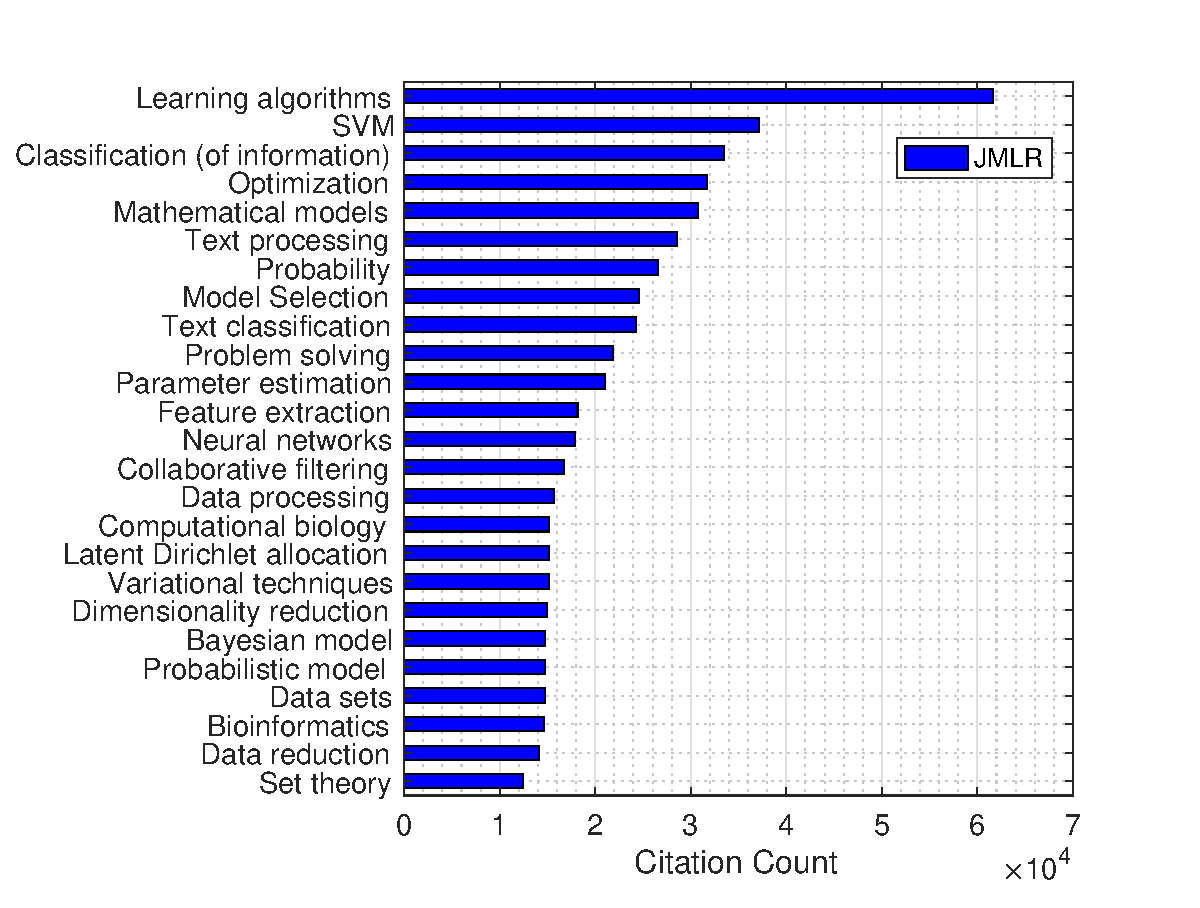
\includegraphics[width=0.45\textwidth]{figure/keywords_cite_JMLR.eps}}\\
		\subfloat[]{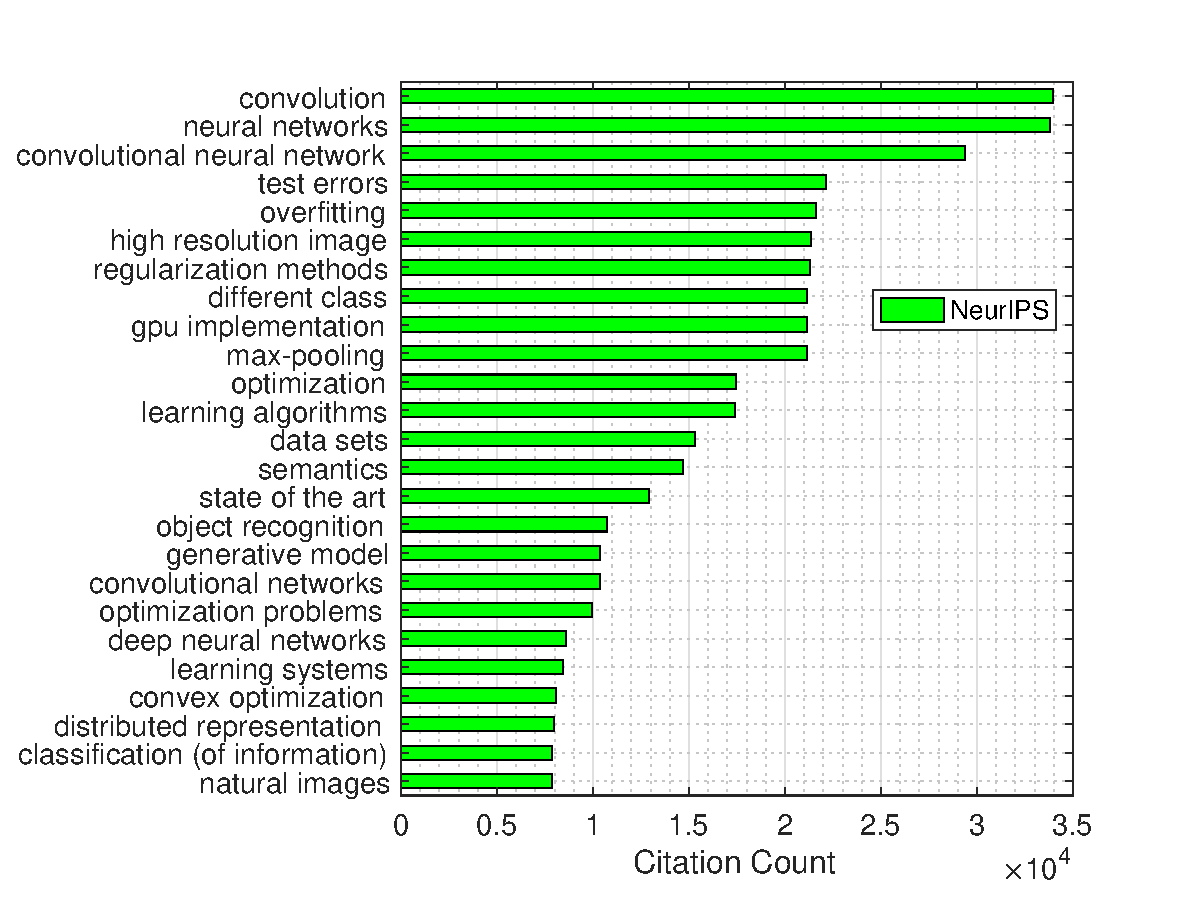
\includegraphics[width=0.45\textwidth]{figure/keyword_cite_NIPS.eps}}
	\subfloat[]{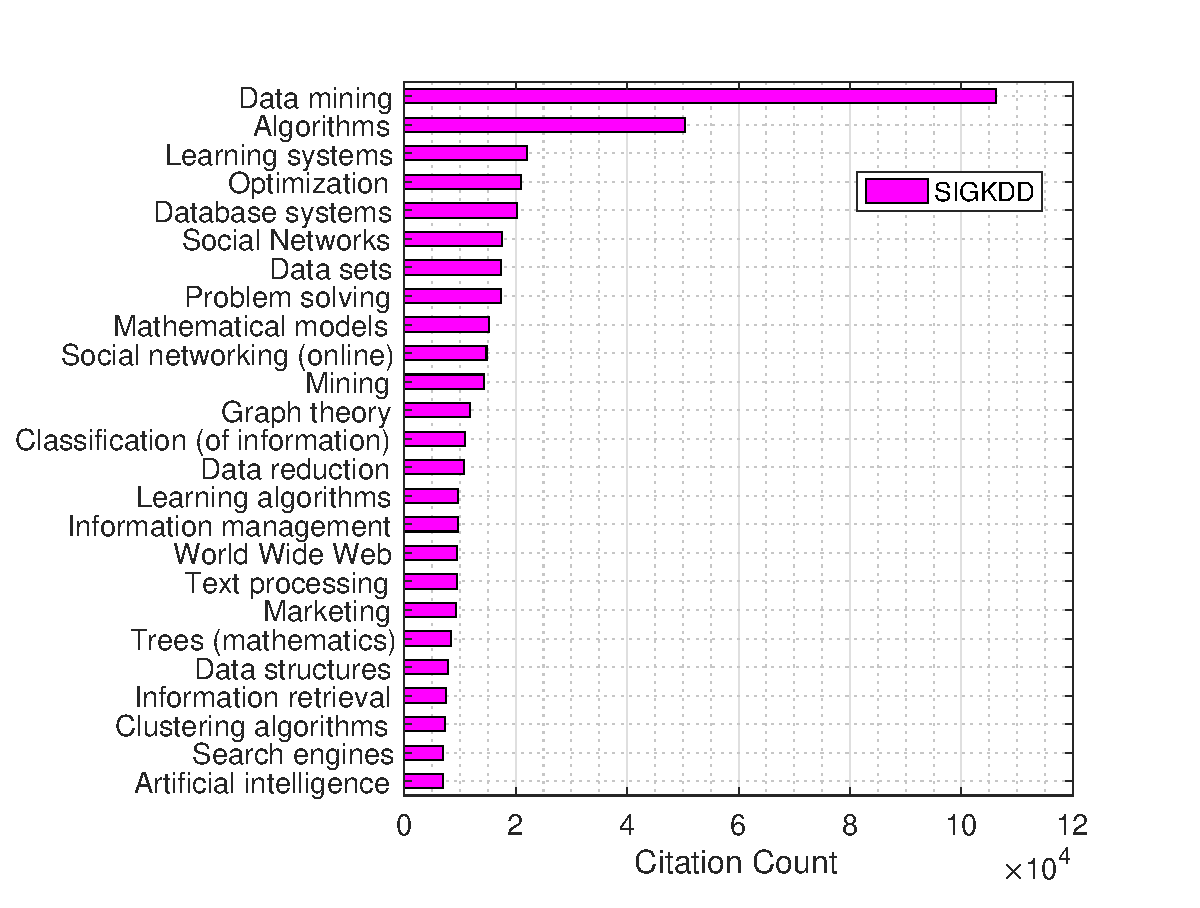
\includegraphics[width=0.45\textwidth]{figure/keyword_cite_SIGKDD.eps}}
	\end{center}
	\caption{Most-cited keywords. \textit{It is noticeable that there is negligible overlap in the keywords used in all discussed venues.}}
	\label{fig:cited_top_keywords}
\end{figure*}
